\documentclass[11pt,a4paper]{article}

\usepackage[margin=2.4cm,top=2.6cm,bottom=2.6cm]{geometry}
\usepackage{fontspec}
\usepackage{booktabs}
\usepackage{graphicx}
\usepackage{xcolor}
\usepackage{titlesec}
\usepackage{caption}
\usepackage{array}
\usepackage{enumitem}
\usepackage{amsmath}
\usepackage[hidelinks]{hyperref}
\usepackage{fancyhdr}

\setmainfont{Palatino}
\setsansfont{Helvetica Neue}[Scale=MatchLowercase]
\setmonofont{Menlo}[Scale=0.85]

\definecolor{ink}{HTML}{0B0B0B}
\definecolor{ink2}{HTML}{52514E}
\definecolor{muted}{HTML}{898781}
\definecolor{accent}{HTML}{2A78D6}

\titleformat{\section}{\sffamily\Large\bfseries\color{ink}}{\thesection}{0.7em}{}
\titleformat{\subsection}{\sffamily\large\bfseries\color{ink}}{\thesubsection}{0.6em}{}
\titlespacing*{\section}{0pt}{2.2ex plus 1ex minus .2ex}{1.1ex plus .2ex}

\captionsetup{font={sf,small,color=ink2},labelfont={bf},skip=6pt}
\setlength{\parskip}{0.62em}
\setlength{\parindent}{0pt}
\renewcommand{\arraystretch}{1.15}

\pagestyle{fancy}
\fancyhf{}
\renewcommand{\headrulewidth}{0.4pt}
\fancyhead[L]{\sffamily\footnotesize\color{muted}A Stock-Only Quality Strategy}
\fancyhead[R]{\sffamily\footnotesize\color{muted}\thepage}

\newcommand{\keyfinding}[1]{%
  \par\vspace{0.4em}%
  \noindent\colorbox{ink!4}{\parbox{\dimexpr\linewidth-2\fboxsep}{\vspace{0.3em}#1\vspace{0.3em}}}%
  \par\vspace{0.4em}}

\begin{document}

\thispagestyle{empty}
\begin{center}
\vspace*{1.2cm}
{\sffamily\Huge\bfseries A Stock-Only\\[0.15em] Quality Strategy}\\[0.5em]
{\sffamily\Large\color{ink2} Twenty businesses, no leverage, no funds,\\ no market timing}\\[1.4em]
{\sffamily\large\color{muted} What survives when the toolkit is individual common stock}\\[0.8em]
{\sffamily\normalsize\color{muted} Investa research note \quad\textbullet\quad 29 July 2026}
\end{center}

\vspace{1.2cm}
\hrule height 0.4pt
\vspace{0.9em}

\section*{\sffamily Executive summary}

This note supersedes two earlier drafts. The first paired the Buffett quality
ranking with a 2$\times$ leveraged NASDAQ sleeve; the second removed the
leverage. This one removes index funds as well, at the reader's instruction.
What is left is a portfolio of individual companies, and the honest conclusion
is that the removals cost real return while leaving a defensible strategy.

\begin{enumerate}[leftmargin=1.4em,itemsep=0.35em]
  \item \textbf{The strategy is now a single rule.} Hold the top 20 companies
  by the 80/20 quality--value composite, equally weighted, capped at three
  names per industry, rebalanced each January. Nothing else: no leverage, no
  index or cash ETF, no timing overlay, and no defensive mode.

  \item \textbf{Over 2013--2025 it returned 17.4\% a year} (\$1 $\rightarrow$
  \$8.1) against 14.7\% for the S\&P 500 total return and \textbf{14.7\% for
  the portfolio's own time-weighted return}. It clears both of those bars.

  \item \textbf{The discounted-cash-flow term has been removed from the
  ranking} (\S\ref{sec:nodcf}). It was measured against thirteen years of
  point-in-time rankings and found to be noise; cutting it, and the three
  further multiples that measured no better, raised the return from 16.3\% to
  17.4\%, lifted the Sharpe from 0.95 to 1.05 and cut the worst drawdown from
  $-24.3\%$ to $-21.5\%$.

  \item \textbf{It still does not beat the NASDAQ-100} (19.7\%), though it is
  now close on risk-adjusted terms: Sharpe 1.05 against the NASDAQ's 1.15 and
  the S\&P's 1.04. Without a second, differently behaved sleeve there is
  nothing to damp the swings.

  \item \textbf{The trend filter had to go, and the measurement says it should
  have.} With no index fund to hold, the only surviving use of the signal was
  to move the \emph{stock} book to cash. Tested, that returns 13.0\% instead of
  16.3\% \emph{and} deepens the worst drawdown to $-27.9\%$ from $-24.3\%$
  (\S\ref{sec:filter}); both figures were measured on the ranking as it stood
  before the DCF was removed and have not been re-run, the conclusion not being
  close. It is kept in the app as a market-context indicator that no strategy
  acts on.

  \item \textbf{Three alternatives are shipped alongside} for different
  appetites (\S\ref{sec:variants}), but they are variations on one idea. There
  is no longer a diversifying second engine, and the report is explicit about
  what that costs.
\end{enumerate}

\section{The bars to clear}

Measured over 2013--2025, the window set by the point-in-time floor of the
EDGAR fundamentals:

\begin{table}[!ht]
\centering\sffamily\small
\begin{tabular}{lrrrr}
\toprule
 & CAGR & Volatility & Max drawdown & Sharpe \\
\midrule
\textbf{Buffett Quality 20} & \textbf{17.4\%} & 16.5\% & $-21.5\%$ & 1.05 \\
NASDAQ-100 (QQQ, TR) & 19.7\% & 17.2\% & $-32.6\%$ & 1.15 \\
S\&P 500 (SPY, TR) & 14.7\% & 14.2\% & $-23.9\%$ & 1.04 \\
My portfolio (time-weighted) & 14.7\% & 18.5\% & $-24.6\%$ & 0.80 \\
\bottomrule
\end{tabular}
\caption{The strategy beats the S\&P 500 on return and matches it on risk, and
beats the portfolio on both. It still trails the NASDAQ-100 on return, though
its worst drawdown is a third shallower. The
portfolio's full-history TWR (2003--2025) is 18.1\%/yr, which nothing in this
note matches.}
\end{table}

\begin{figure}[!ht]
\centering
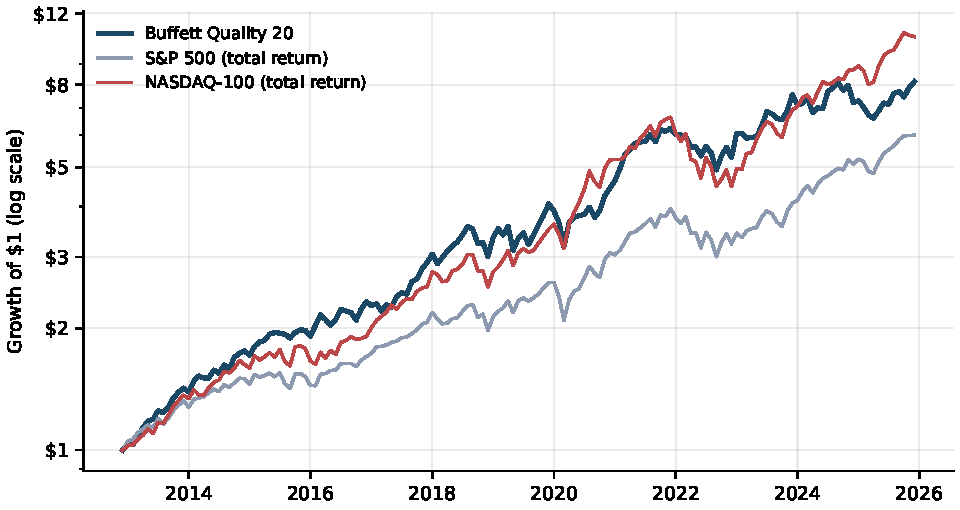
\includegraphics[width=\linewidth]{figures/fig_quality_growth.pdf}
\caption{Growth of \$1, January 2013 -- December 2025, month-end data, log
scale. The strategy (\textcolor{accent}{\textbf{blue}}) tracks the NASDAQ
closely until 2020 and falls behind through the 2021--2025 mega-cap run.}
\end{figure}

\section{The rule}

\keyfinding{\textbf{Buffett Quality 20.} Each January, rank every US-listed
company with sufficient filing history on an 80/20 blend of business quality
and valuation, scored point-in-time from SEC EDGAR. Buy the top 20, equally
weighted at 5\% each, taking no more than three names from any 2-digit
industry group. Hold for the year. Sell nothing in between.\\[0.45em]
\textbf{The constraints, all structural:} no leverage, no margin, no index
funds, no ETFs of any kind, no cash sleeve. The book is twenty companies and
nothing else.}

The industry cap is the one discretionary choice. Without it the ranking would
currently hold six banks and three mortgage insurers --- 45\% of the book on
one correlated balance-sheet risk, and in the exact cohort where the
survivorship bias bites hardest, since post-2009 mortgage insurers are the
survivors of a sector that was largely destroyed. The cap costs 0.2 points of
backtested CAGR (17.4\% against 17.6\%) and is the better trade in a live book.

\begin{figure}[!ht]
\centering
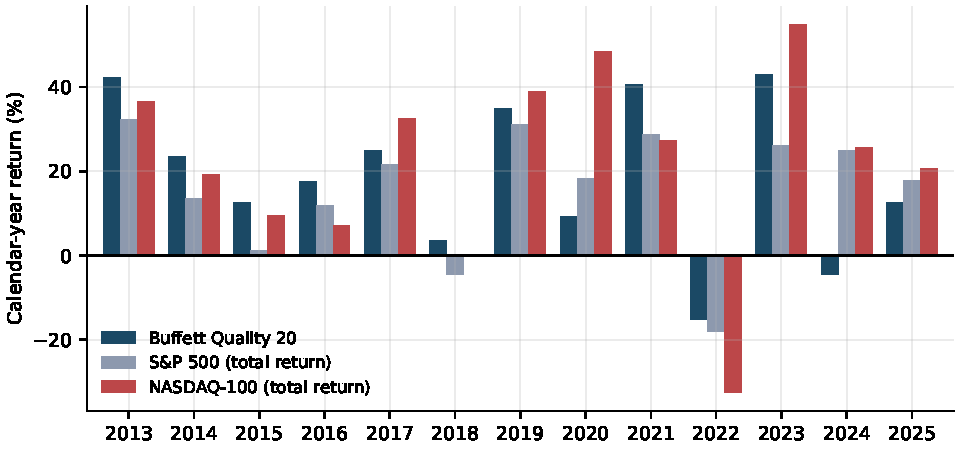
\includegraphics[width=\linewidth]{figures/fig_quality_annual.pdf}
\caption{Calendar-year returns. Note 2022 ($-15.3\%$ against the NASDAQ's
$-32.6\%$) and 2024 ($-4.5\%$ against $+25.6\%$): the strategy is a genuinely
different portfolio, which cuts both ways.}
\end{figure}

\section{Why the DCF was removed}\label{sec:nodcf}

The value half of the ranking used to be led by a \emph{margin of safety}: the
gap between the price and a discounted-cash-flow valuation, taken at the 25th
percentile of a Monte Carlo distribution so as to be conservative. It carried
35\% of the value score. It is gone, and the case for removing it is a
measurement rather than a preference.

Each signal in the ranking was scored by its information coefficient --- the
rank correlation between the signal and the \emph{next} year's total return,
computed across the universe in each of the thirteen rebalance years. The
margin of safety scored $+1.7\%$ with a $t$-statistic of 1.05 and a hit rate of
54\%: indistinguishable from a coin. Worse, its sign was unstable, essentially
zero over 2013--19 and positive only over 2020--25.

Three further facts settled it:

\begin{itemize}[leftmargin=1.4em,itemsep=0.3em]
  \item \textbf{The valuations were not credible.} The median eligible company
  scored a margin of safety of $-33\%$ and the 10th percentile around $-500\%$.
  The model was asserting that the typical listed business is worth a third of
  its market price, which is not a valuation but a broken one.

  \item \textbf{Ranking on it lost money relative to doing nothing.} Buying the
  top 20 companies by margin of safety alone compounded at 9.7\%/yr against
  12.25\% for the average of the whole eligible universe.

  \item \textbf{It was mostly a noisy restatement of the earnings yield}, with
  which it correlated 0.58 --- and the earnings yield is in the ranking already,
  costs nothing to compute, and measures three times better.
\end{itemize}

Buying the estimate from a data vendor was considered and rejected: published
third-party DCFs show the same pathology, putting Amazon at \$72 against a \$231
price and Alphabet at \$128 against \$334, and analyst consensus price targets
correlate 0.972 with the current price, making them price in a hat rather than
an independent check on it. The failure is in the model class, not in whose
arithmetic runs it.

Removing the DCF made the remaining multiples measurable for the first time,
and three of the five did not survive either. Price-to-book scored $-1.4\%$,
negative in \emph{both} windows; EV/EBIT and price-to-sales scored around zero
with unstable signs. Only the earnings yield ($+3.5\%$, positive in both
windows) and the free-cash-flow yield were kept, weighted 60/40 --- a ratio
chosen from the middle of a broad 0.50--0.70 plateau rather than from the
grid's best cell. Cutting the three weak multiples improved the Sharpe ratio,
the drawdown and the held-out return in three of three strategy shapes tested.

\keyfinding{The net effect on the default strategy: CAGR 16.3\% $\rightarrow$
\textbf{17.4\%}, Sharpe 0.95 $\rightarrow$ \textbf{1.05}, worst drawdown
$-24.3\%$ $\rightarrow$ $\mathbf{-21.5\%}$. The held-out window is the one
figure that did not improve (12.9\% $\rightarrow$ 12.1\%), and it remains the
weakest part of the whole case.}

The valuation models themselves are untouched and still power the per-stock
screener and stock-detail views, where a reader is deliberately inspecting one
company's assumptions. What changed is that a \emph{cross-sectional ranking} no
longer rests on them.

\section{Why the trend filter was dropped}\label{sec:filter}

The two earlier drafts used a 10-month moving-average signal to decide whether
to hold a NASDAQ position. With index funds excluded there is no such position,
so the only remaining use was to sell the \emph{stocks} when the market turned
down and sit in cash. That was tested rather than assumed.

\begin{figure}[!ht]
\centering
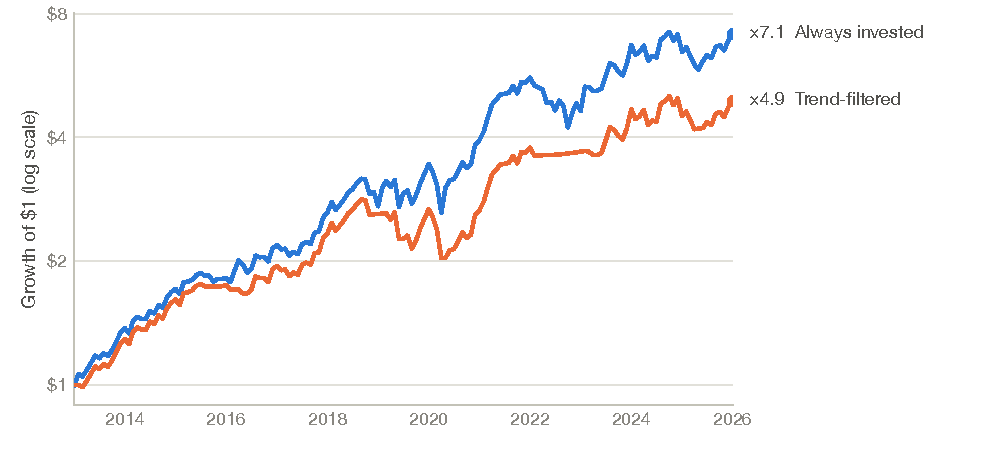
\includegraphics[width=\linewidth]{figures/fig_trend_filter_rejected.pdf}
\caption{The same twenty-stock book, held through everything against gated by
the market's 10-month trend. Filtering cost a third of the terminal value.
Measured on the ranking as it stood before the DCF was removed
(\S\ref{sec:nodcf}); the gap is far too wide for that to change the verdict.}
\end{figure}

\begin{table}[!ht]
\centering\sffamily\small
\begin{tabular}{lrrrr}
\toprule
2013--2025 & CAGR & Max drawdown & Sharpe & Growth of \$1 \\
\midrule
\textbf{Always invested} & \textbf{16.3\%} & $\mathbf{-24.3\%}$ & \textbf{0.95} & \textbf{\$7.1} \\
Trend-filtered to cash & 13.0\% & $-27.9\%$ & 0.91 & \$4.9 \\
\bottomrule
\end{tabular}
\caption{The filter loses on every measure at once --- including the drawdown
it was supposed to reduce.}
\end{table}

It helped in three years of thirteen (2015, 2018, 2022) and hurt in six, worst
in 2019 (2.7\% against 26.6\%) and 2020 ($-0.6\%$ against 14.3\%). The reason
is a mismatch rather than bad luck: the signal describes the NASDAQ, while the
book is twenty value-weighted businesses that correlate with it at 0.46. Timing
one asset with a signal about another sells after declines the book did not
share and buys back after recoveries it already had.

\textbf{The indicator is still in the app}, on the dashboard, clearly labelled
as market context. Its payload carries an explicit \texttt{advisory\_only}
flag, and no strategy reads it.

\section{The variants}\label{sec:variants}

Four rules ship, all of them the same idea at different settings:

\begin{table}[!ht]
\centering\sffamily\small
\begin{tabular}{lrrrrr}
\toprule
 & CAGR & Max DD & Sharpe & Train & Test \\
 & & & & 2013--19 & 2020--25 \\
\midrule
\textbf{Buffett Quality 20} (default) & \textbf{17.4\%} & $-21.5\%$ & 1.05 & 21.9\% & 12.1\% \\
Quality 20, uncapped & 17.6\% & $-20.0\%$ & 1.08 & 21.4\% & 13.0\% \\
Quality 15 & 18.9\% & $-18.8\%$ & 1.11 & 21.3\% & 15.9\% \\
Quality, price-blind (100\% quality) & 15.9\% & $-20.3\%$ & 1.07 & 20.0\% & 11.0\% \\
\bottomrule
\end{tabular}
\caption{The uncapped list returns more but concentrates in financials; the
15-name book returns the same as the uncapped 20 with a deeper worst case; the
price-blind variant is the steadiest but has the weakest held-out return.}
\end{table}

Two findings constrain the choice and are worth not re-deriving. The quality
weight improves results monotonically from 0\% to 80\% in both windows, but
100\% (ignoring price entirely) degrades out of sample --- which is why the
price-blind variant, despite the best Sharpe, is not the default. And
concentration is a plateau from roughly 10 to 20 names; below that the results
become unstable.

\section{Risks, stated plainly}

\begin{itemize}[leftmargin=1.4em,itemsep=0.3em]
  \item \textbf{Always fully invested.} There is no defensive mode. A
  market-wide fall is taken in full, and the 2022 drawdown of $-21.5\%$ is the
  worst \emph{measured}, not a bound.
  \item \textbf{Weak out of sample.} The strategy returned 19.3\% in the
  training window and 12.9\% in the held-out one. That gap is the largest of
  anything in these three notes, and the earlier drafts used a second sleeve
  precisely to damp it. That option is now gone.
  \item \textbf{Survivorship bias, unhedged.} The universe is built from
  today's listing files, so companies that were delisted, acquired or went
  bankrupt never appear as candidates. The benchmarks carry no such bias, so
  the 17.4\% is flattered by an unknown amount and the true edge over the S\&P
  is smaller than 1.5 points.
  \item \textbf{Twenty names is real single-stock risk.} One blow-up costs 5\%
  of the book with no index diversification behind it.
  \item \textbf{Concentration by construction.} Even capped, the current list
  is 15\% mortgage insurance, 15\% banks and 15\% homebuilders --- 45\% tied
  to the interest-rate cycle.
  \item \textbf{Taxes not modelled.} The January rebalance turns over roughly
  half the book and realises gains annually.
\end{itemize}

\section{The portfolio, as of 29 July 2026}\label{sec:portfolio}

Sizing uses the portfolio's current market value of \textbf{\$1{,}779{,}662}
(Investa, 28 July 2026 close), all of it in one sleeve. Every figure scales
linearly.

From ranking run \#11 (29 July 2026, 1{,}244 companies scored on filings
through the June quarter --- the first run under the DCF-free value score):

\begin{table}[!ht]
\centering\sffamily\footnotesize
\begin{tabular}{llrrrr}
\toprule
Symbol & Industry & Price & Shares & Cost & Weight \\
\midrule
MTG (MGIC Investment) & Mortgage insurance & 30.61 & 2{,}906 & \$88{,}953 & 5.0\% \\
UNTY (Unity Bancorp) & Banks & 58.91 & 1{,}510 & \$88{,}959 & 5.0\% \\
RDN (Radian Group) & Mortgage insurance & 39.51 & 2{,}252 & \$88{,}977 & 5.0\% \\
LULU (lululemon) & Apparel & 119.19 & 746 & \$88{,}919 & 5.0\% \\
TSBK (Timberland Bancorp) & Banks & 45.06 & 1{,}974 & \$88{,}948 & 5.0\% \\
ESNT (Essent Group) & Mortgage insurance & 67.54 & 1{,}317 & \$88{,}950 & 5.0\% \\
BSVN (Bank7) & Banks & 50.30 & 1{,}769 & \$88{,}981 & 5.0\% \\
INVA (Innoviva) & Pharma & 21.81 & 4{,}080 & \$88{,}964 & 5.0\% \\
ADBE (Adobe) & Software & 257.04 & 346 & \$88{,}934 & 5.0\% \\
NVR (NVR) & Homebuilders & 6{,}459.99 & 13 & \$83{,}980 & 4.7\% \\
PHM (PulteGroup) & Homebuilders & 133.66 & 665 & \$88{,}884 & 5.0\% \\
ACN (Accenture) & IT services & 169.41 & 525 & \$88{,}940 & 5.0\% \\
GOOG (Alphabet C) & Software & 332.57 & 267 & \$88{,}796 & 5.0\% \\
ZTS (Zoetis) & Pharma & 78.81 & 1{,}129 & \$88{,}976 & 5.0\% \\
G (Genpact) & Consulting & 35.91 & 2{,}477 & \$88{,}949 & 5.0\% \\
CPRT (Copart) & Auto auctions & 30.81 & 2{,}888 & \$88{,}979 & 5.0\% \\
AGM (Farmer Mac) & Credit & 213.45 & 416 & \$88{,}795 & 5.0\% \\
TOL (Toll Brothers) & Homebuilders & 151.46 & 587 & \$88{,}907 & 5.0\% \\
DECK (Deckers) & Footwear & 103.01 & 863 & \$88{,}902 & 5.0\% \\
XPEL (XPEL) & Auto films & 44.33 & 2{,}007 & \$88{,}980 & 5.0\% \\
\bottomrule
\end{tabular}
\caption{The full book at 29 July 2026 quotes: \$1{,}773{,}675 invested,
\$5{,}987 residual cash. Prices move, so share counts are indicative; the fixed
part of the rule is the equal 5\% weights.}
\label{tab:buylist}
\end{table}

\section{The operating plan}\label{sec:plan}

Removing the trend sleeve removed the monthly routine with it. What remains is
an annual rule and a short list of things not to do.

\subsection{Today}

\begin{enumerate}[leftmargin=1.6em,itemsep=0.25em]
  \item Buy the twenty names in Table~\ref{tab:buylist} at market, equal 5\%
  weights.
  \item Note the January rebalance anniversary. That is the only recurring task.
\end{enumerate}

\subsection{Every January}

\begin{enumerate}[leftmargin=1.6em,itemsep=0.25em]
  \item Open Investa's \textsf{Strategies} tab, or run
  \texttt{python scripts/buffett\_live\_picks.py --quality 0.8
  --max-per-sector 3 --sector-digits 2} with the book's current value.
  \item Sell the names that dropped out of the new top twenty; buy the
  entrants; trim or add the holdovers back to equal 5\% weights. Historically
  about half the book turns over.
  \item Do not carry opinions across the rebalance: a name that fell to \#23 is
  sold even if it is loved, a name at \#4 is bought even if it is boring. The
  ranking already encodes the thesis.
\end{enumerate}

\subsection{The rest of the year --- what not to do}

\begin{itemize}[leftmargin=1.4em,itemsep=0.25em]
  \item \textbf{A holding crashes on news:} nothing. There are no stop-losses;
  single-name risk is what the twenty-way split and the January re-rank are for.
  \item \textbf{The market falls:} nothing. This is the consequence of having
  no defensive sleeve, and it was measured: the version that sold into cash did
  worse on return \emph{and} drawdown.
  \item \textbf{The dashboard's market-trend card turns down:} nothing. It is
  context, not an instruction, and acting on it is the strategy
  \S\ref{sec:filter} rejected.
  \item \textbf{A holding is acquired or delisted:} keep the proceeds as cash
  until January rather than replacing it mid-year.
  \item \textbf{Splits, spin-offs, special dividends:} hold what is received;
  true up at the next January.
\end{itemize}

\subsection{What to expect --- agreed in advance}

\begin{itemize}[leftmargin=1.4em,itemsep=0.25em]
  \item \textbf{Full participation in every market decline}, including the next
  one deeper than $-24\%$.
  \item \textbf{Whole years of underperformance.} 2024 returned $-3.7\%$ while
  the NASDAQ made 25.6\%. Two or three such years in a row are consistent with
  the strategy working.
  \item \textbf{An unfashionable book.} Mortgage insurers and micro-cap banks
  will rarely feel comfortable to own. They are there because fifteen years of
  filings say the businesses compound.
\end{itemize}

\textbf{When to actually worry} (reviewed each January): lagging the S\&P 500
over three consecutive January-to-January years; the industry cap binding so
hard that the book stops resembling the ranking; or a structural change in
EDGAR coverage. Any of those triggers a re-run of the backtests, not an
improvised exit.

\vspace{0.6em}
{\sloppy Reproduction: \texttt{buffett\_strategy\_search.py} and
\texttt{buffett\_live\_picks.py} in \texttt{scripts/}, run from the repo root
against cached data. The strategies are implemented in
\texttt{src/strategies.py} and shipped in all three Investa clients.\par}

\par\nopagebreak\vspace{0.5em}
{\sffamily\footnotesize\color{muted}
Sources: SEC EDGAR XBRL point-in-time fundamentals (ranking run \#4, 28 July
2026); Yahoo Finance prices; the Investa transaction database for the
portfolio's time-weighted returns and current value. Past performance,
simulated or realized, does not guarantee future results.}

\end{document}
